% T28 | Responsable: Rhamses (R6) | Informe final en formato IEEE (borrador).
% Compilar desde reports/informe con:  latexmk -pdf -interaction=nonstopmode main.tex
% Las figuras se leen de ../../results/figures/, por lo que debe montarse la raíz del repositorio.
% Marcadores pendientes: buscar «TODO-» (rg -n "TODO-" reports/informe).
\documentclass[conference,a4paper]{IEEEtran}

\usepackage[utf8]{inputenc}
\usepackage[T1]{fontenc}
\usepackage[spanish,es-tabla,es-noshorthands]{babel}
\usepackage{amsmath,amssymb}
\usepackage{graphicx}
\usepackage{booktabs}
\usepackage{multirow}
\usepackage{siunitx}
\usepackage{url}
\usepackage[hidelinks]{hyperref}

\sisetup{output-decimal-marker={,}, group-separator={\,}, group-minimum-digits=4, group-digits=integer}

% Rutas relativas a reports/informe.
\graphicspath{{../../results/figures/}}

% Notación común.
\newcommand{\phat}{\hat{p}}
\newcommand{\Amax}{A_{\max}}
\newcommand{\codigo}[1]{\texttt{#1}}

\begin{document}

\title{Estimación paralela del riesgo de inundación urbana ante lluvias mediante simulación Monte Carlo distribuida}

% TODO-T46: completar apellidos y correos institucionales de los integrantes.
\author{\IEEEauthorblockN{David, Angela, Ashley, Lita, Miguel y Rhamses}
\IEEEauthorblockA{Grupo 8 --- Programación Concurrente y Paralela\\
Facultad de Ingeniería de Sistemas e Informática\\
Universidad Nacional Mayor de San Marcos, Lima, Perú}}

\maketitle

\begin{abstract}
Se presenta un simulador Monte Carlo, escrito en C++17, que estima la probabilidad de que el agua acumulada en una zona urbana supere un umbral crítico durante una temporada de lluvias, en función de la capacidad de drenaje. La lluvia diaria se genera con una cadena de Markov de dos estados y montos gamma calibrados con series del SENAMHI para estaciones de la costa norte y de Lima, separando años normales y años El Niño según el Índice Costero El Niño. La acumulación sigue la recursión de Lindley. El cómputo se paraleliza con OpenMP, con MPI en dos esquemas (reparto estático con reducción y maestro--trabajador dinámico) y con un esquema híbrido MPI + OpenMP, desplegados en contenedores Docker sobre Compose y Swarm. Un generador Philox basado en contador hace que todos los backends produzcan conteos idénticos bit a bit. En el equipo de referencia, con $N = 2\times10^{7}$ temporadas, la versión secuencial tarda \qty{59.70}{\second} y OpenMP con 16 hilos alcanza un speedup de \num{10.94}.
% TODO-T46: completar el resumen con MPI, híbrido, X1--X3 y los resultados científicos (T33, T35, T42).
\end{abstract}

\begin{IEEEkeywords}
Monte Carlo, OpenMP, MPI, programación híbrida, generador basado en contador, riesgo de inundación, El Niño.
\end{IEEEkeywords}

\section{Introducción}
\label{sec:introduccion}

\IEEEPARstart{L}{as} lluvias asociadas a El Niño costero producen inundaciones recurrentes en Piura y Tumbes, mientras que en Lima una llovizna moderada puede colapsar los desagües de distritos cuyo drenaje pluvial es casi inexistente. En ambos casos la variable decisiva no es solo la cantidad de lluvia, sino la relación entre el agua que cae, el agua que el sistema puede evacuar por día y la persistencia de los días lluviosos. Esa relación puede cuantificarse: conocida la estadística de la lluvia diaria y una capacidad de drenaje, se puede estimar con qué frecuencia la primera supera a la segunda.

Este trabajo construye un simulador que responde tres preguntas para cada zona estudiada: (i) cuál es la probabilidad de que ocurra al menos un evento de inundación en una temporada de lluvias; (ii) cuánto disminuye esa probabilidad al aumentar la capacidad de drenaje y cuál es la capacidad mínima que la mantiene por debajo de un umbral de diseño; y (iii) cuánto cambia el riesgo en un año El Niño frente a un año normal. El sistema no pronostica el clima ni modela la hidráulica de la red: estima probabilidades por temporada a partir de un modelo estocástico calibrado con datos públicos.

La estimación es de tipo Monte Carlo y su precisión crece con el número de temporadas simuladas. Cubrir 5 estaciones, 2 regímenes climáticos, 13 capacidades de drenaje y 100 conjuntos de parámetros obtenidos por remuestreo, con $10^{6}$ temporadas por combinación, exige del orden de $1{,}3\times10^{10}$ temporadas de 120 días. Las temporadas son independientes entre sí, por lo que el problema es \emph{embarazosamente paralelo}; el interés técnico está en repartir el trabajo entre hilos, procesos y equipos sin alterar el resultado y en medir con rigor la ganancia obtenida.

Las contribuciones del trabajo son:
\begin{itemize}
  \item un núcleo de simulación determinista cuyo resultado depende solo de los parámetros, la semilla y el índice global del escenario, gracias al generador Philox4x32-10 basado en contador~\cite{salmon2011};
  \item cinco implementaciones (secuencial, OpenMP, MPI estático, MPI dinámico e híbrida MPI + OpenMP) con conteos idénticos bit a bit, verificados de forma automática;
  \item un despliegue reproducible en contenedores Docker, con Compose para las pruebas en un equipo y Swarm para el clúster de tres equipos físicos;
  \item una campaña de rendimiento con calentamiento y cinco repeticiones por punto, que informa tiempo, speedup, eficiencia, throughput y fracción serial de Karp--Flatt~\cite{karp1990}.
\end{itemize}

La Sección~\ref{sec:problema} plantea el problema y su dimensionamiento; la Sección~\ref{sec:modelo}, el modelo de simulación; la Sección~\ref{sec:metodologia}, la metodología de verificación y medición; las Secciones~\ref{sec:entorno} y~\ref{sec:implementacion}, el entorno y las implementaciones; la Sección~\ref{sec:rendimiento}, los resultados de rendimiento; las Secciones~\ref{sec:resultados} y~\ref{sec:sensibilidad}, los resultados científicos y la sensibilidad; y la Sección~\ref{sec:conclusiones}, las conclusiones.

\section{Planteamiento del problema}
\label{sec:problema}

\subsection{Contexto}

La costa del Perú presenta dos mecanismos de inundación por lluvia. En la costa norte (Piura, Tumbes), el calentamiento anómalo del mar durante El Niño costero dispara convección sobre la llanura costera y produce lluvias extremas entre enero y abril; el riesgo está dominado por la \emph{cantidad} de lluvia. En Lima la lluvia es casi nula en un año normal, pero la capacidad de drenaje urbano es tan baja que lluvias moderadas bastan para causar daños; el riesgo está dominado por la \emph{capacidad de evacuación}. Un modelo útil debe capturar ambos casos con los mismos parámetros físicos: lluvia diaria, capacidad de drenaje y umbral crítico de acumulación.

\subsection{Zonas y regímenes climáticos}

Las series diarias de precipitación provienen del portal de datos hidrometeorológicos del SENAMHI~\cite{senamhi}. Se auditaron 8 estaciones de la costa norte y de Lima. Una combinación estación--año es elegible si tiene menos del 10\,\% de días faltantes en la temporada de su zona y no presenta valores negativos sin corregir. Con ese criterio se eligieron 5 estaciones de trabajo: Miraflores y Bernal (Piura), Puerto Pizarro y El Tigre (Tumbes) y Chosica (Lima), todas con al menos 20 años elegibles. La temporada es enero--abril en la costa norte y en Chosica, cuyo régimen de lluvias es convectivo de verano y no de garúa costera.

Cada año se clasifica como \emph{normal} o \emph{El Niño} con la definición operacional del ENFEN~\cite{enfen2012}: un mes es cálido si el Índice Costero El Niño (ICEN)~\cite{icen} supera \num{0.4}, y hay un evento El Niño cuando se encadenan al menos tres meses cálidos consecutivos. Un año se clasifica como El Niño si alguno de los meses de su temporada pertenece a un evento. Cada régimen se calibra y se simula por separado, lo que permite responder la pregunta (iii) de la Sección~\ref{sec:introduccion}.

\subsection{Qué es un dato y cuánto cómputo exige}

El dato elemental es un \emph{día-escenario}: un día de lluvia sintética generado y procesado por la recursión del balance hídrico. Una temporada contiene $D = 120$ días-escenario. La Tabla~\ref{tab:dimensionamiento} resume la carga oficial, que combina incertidumbre de muestreo (temporadas por conjunto) e incertidumbre de calibración (conjuntos bootstrap).

\begin{table}[!t]
\centering
\caption{Dimensionamiento de la carga oficial}
\label{tab:dimensionamiento}
\begin{tabular}{@{}lr@{}}
\toprule
Factor & Cantidad \\
\midrule
Estaciones SENAMHI & 5 \\
Capacidades de drenaje $C$ (5--65~mm/día, paso 5) & 13 \\
Regímenes (normal, El Niño) & 2 \\
Conjuntos de parámetros bootstrap $K$ & 100 \\
Temporadas por conjunto $N$ & $10^{6}$ \\
\midrule
Total de temporadas & $1{,}3\times10^{10}$ \\
Total de días-escenario ($\times 120$) & $1{,}56\times10^{12}$ \\
\bottomrule
\end{tabular}
\end{table}

El costo secuencial medido en el equipo de referencia es de \qty{2.985}{\micro\second} por temporada (Sección~\ref{sec:rendimiento}). Extrapolado linealmente, la carga oficial requiere cerca de \qty{3.9e4}{\second} (\num{10.8}~horas) en un núcleo. Guardar la lluvia simulada en precisión simple ocuparía $1{,}56\times10^{12}\times\qty{4}{\byte} \approx \qty{6.2}{\tera\byte}$; por eso el diseño nunca la almacena: cada temporada se reduce en el momento a un indicador de inundación y a una entrada de un histograma.
% TODO-T34: confirmar la carga efectivamente ejecutada en la corrida oficial X6 y su tiempo real en el clúster.

\subsection{Alcance}

El sistema no es un pronóstico meteorológico ni un modelo hidráulico: no simula topografía, escorrentía ni flujo en tuberías. La capacidad de drenaje y el umbral crítico se tratan como escenarios de diseño barridos en un rango; el rango de $C$ toma como referencia la norma peruana de drenaje pluvial urbano OS.060~\cite{os060}. La simplicidad del modelo físico es deliberada, para aislar el efecto de la paralelización.

\section{Modelo de simulación}
\label{sec:modelo}

\subsection{Unidad de simulación}

Un \emph{escenario} es una temporada de lluvias hipotética de $D$ días, generada al azar pero coherente con la estadística observada de la zona y el régimen. Cada escenario produce dos salidas: un veredicto binario (inundación o no) y el máximo de agua acumulada $\Amax$ durante la temporada. La Tabla~\ref{tab:parametros} resume los parámetros.

\begin{table}[!t]
\centering
\caption{Parámetros del modelo}
\label{tab:parametros}
\begin{tabular}{@{}llr@{}}
\toprule
Símbolo & Descripción & Origen / valor \\
\midrule
$D$ & Días de la temporada & 120 \\
$p_{01}$ & $P(\text{lluvia hoy} \mid \text{ayer seco})$ & Calibrado \\
$p_{11}$ & $P(\text{lluvia hoy} \mid \text{ayer lluvioso})$ & Calibrado \\
$\alpha,\theta$ & Forma y escala (mm) de la gamma & Calibrados (Thom) \\
$C$ & Capacidad de drenaje (mm/día) & 5--65, paso 5 \\
$U$ & Umbral crítico (mm) & 30 / 50 / 80 \\
$K$ & Conjuntos bootstrap & 100 \\
$N$ & Temporadas por conjunto & $10^{6}$ \\
$s$ & Semilla global (64 bits) & Registrada \\
\bottomrule
\end{tabular}
\end{table}

\subsection{Ocurrencia: cadena de Markov de dos estados}

Si la ocurrencia de lluvia fuese independiente día a día, el modelo subestimaría las rachas húmedas, que son las que acumulan agua. Por eso se usa una cadena de Markov de primer orden~\cite{richardson1981,wilks2011}: la probabilidad de lluvia hoy depende solo de si llovió ayer, con $p_{01}$ si ayer fue seco y $p_{11}$ si fue lluvioso. Con $p_{11} > p_{01}$ el modelo reproduce la persistencia observada. La frecuencia estacionaria de días lluviosos es
\begin{equation}
\pi_1 = \frac{p_{01}}{1 - p_{11} + p_{01}}.
\label{eq:estacionaria}
\end{equation}
El día previo a la temporada se toma como seco.

\subsection{Monto: distribución gamma}

En un día lluvioso la lámina $R$ sigue una distribución $\Gamma(\alpha,\theta)$, asimétrica a la derecha: muchos días de lluvia leve y pocos extremos. Se muestrea con el método de Marsaglia y Tsang~\cite{marsaglia2000}. Cuando $\alpha < 1$ se usa la identidad $X = Y\,V^{1/\alpha}$, con $Y\sim\Gamma(\alpha+1,\theta)$ y $V$ uniforme en $(0,1)$.

\subsection{Balance hídrico}

Con capacidad de drenaje $C$ (mm/día) y umbral crítico $U$ (mm), el agua acumulada evoluciona según la recursión de Lindley~\cite{lindley1952}:
\begin{align}
A_0 &= 0, \nonumber\\
A_t &= \max(0,\; A_{t-1} + R_t - C), \qquad t = 1,\dots,D, \label{eq:lindley}\\
\Amax &= \max_{1\le t\le D} A_t, \qquad \text{inundación} \iff \Amax > U. \nonumber
\end{align}
Si el drenaje evacúa todo, el acumulado vuelve a cero; si la lluvia lo supera, el excedente se arrastra al día siguiente. Así, varios días seguidos de lluvia moderada pueden ser más peligrosos que un solo día intenso. La recursión es una caminata aleatoria con barrera reflectante en cero; las temporadas son caminatas independientes, que es la fuente de paralelismo explotada aquí~\cite{youssef1993}.

\subsection{Calibración}

Para cada estación y régimen se usan solo los días de la temporada de los años elegibles. Un día es lluvioso si la precipitación es de al menos \qty{0.1}{\milli\metre}. Las probabilidades de transición se estiman por conteo, $\hat p_{01} = n_{01}/(n_{00}+n_{01})$ y $\hat p_{11} = n_{11}/(n_{10}+n_{11})$. Los parámetros de la gamma se estiman con la aproximación de máxima verosimilitud de Thom~\cite{thom1958}:
\begin{equation}
\hat\alpha = \frac{1 + \sqrt{1 + 4A/3}}{4A}, \quad A = \ln\bar{x} - \overline{\ln x}, \quad \hat\theta = \frac{\bar{x}}{\hat\alpha},
\label{eq:thom}
\end{equation}
donde $\bar x$ es la media de los montos de los días lluviosos. La incertidumbre de calibración se representa con $K = 100$ conjuntos de parámetros obtenidos por remuestreo bootstrap~\cite{efron1979} de los \emph{años} de la serie, con semilla fija; remuestrear años completos conserva la dependencia entre días de una misma temporada.

\subsection{Estimadores}

Para una configuración con $N$ temporadas simuladas y $k$ inundaciones, la probabilidad se estima como $\phat = k/N$. Su intervalo de confianza al 95\,\% es el de Wilson~\cite{wilson1927}:
\begin{equation}
\frac{\phat + \frac{z^2}{2N} \pm z\sqrt{\frac{\phat(1-\phat)}{N} + \frac{z^2}{4N^2}}}{1 + \frac{z^2}{N}}, \qquad z = 1{,}96.
\label{eq:wilson}
\end{equation}
Se prefiere al intervalo de Wald porque mantiene una cobertura cercana a la nominal cuando $\phat$ es pequeña o el número de éxitos es bajo~\cite{agresti1998}, que es el caso de las capacidades de drenaje altas. A esta incertidumbre de muestreo se añade una banda epistémica: los percentiles 5 y 95 de $\phat$ entre los $K$ conjuntos bootstrap. Además, cada configuración guarda un histograma de $\Amax$ con 512 clases de \qty{1}{\milli\metre}, $\min(\lfloor\Amax\rfloor, 511)$, del que se obtiene la curva de excedencia. La curva riesgo--capacidad es $\phat$ en función de $C$, por zona y régimen.

\subsection{Pseudocódigo del núcleo}

La función \codigo{simular\_escenario} es pura: depende solo de los parámetros, de la clave derivada de la semilla y la configuración, y del índice global del escenario (Fig.~\ref{alg:escenario}). La sección~\ref{sec:metodologia} explica por qué esa propiedad garantiza la reproducibilidad entre backends.

\begin{figure}[!t]
\centering
\begin{minipage}{0.95\columnwidth}
\small
\begin{tabbing}
\hspace*{1em}\=\hspace*{1em}\=\hspace*{1em}\=\kill
\textbf{función} \codigo{simular\_escenario}(\codigo{p}, \codigo{clave}, \codigo{idx})\\
\> $A \gets 0$;\; $\Amax \gets 0$;\; \codigo{lluvioso} $\gets$ falso\\
\> \textbf{para} $d = 0,\dots,D-1$ \textbf{hacer}\\
\>\> $u \gets \text{Philox}(\codigo{clave}, \{\codigo{idx}, d, 0\})$\\
\>\> \codigo{lluvioso} $\gets u < (\codigo{lluvioso}\; ?\; p_{11} : p_{01})$\\
\>\> $R \gets \codigo{lluvioso}\; ?\; \Gamma(\alpha,\theta;\, \codigo{clave}, \codigo{idx}, d) : 0$\\
\>\> $A \gets \max(0, A + R - C)$;\; $\Amax \gets \max(\Amax, A)$\\
\> \textbf{devolver} $(\Amax > U,\; \Amax)$
\end{tabbing}
\end{minipage}
\caption{Pseudocódigo de la simulación de una temporada (\codigo{src/core/balance\_hidrico.cpp}).}
\label{alg:escenario}
\end{figure}

\section{Metodología}
\label{sec:metodologia}

\subsection{Números aleatorios basados en contador}

Un programa paralelo puede ser rápido y estar equivocado. En Monte Carlo, un flujo aleatorio sembrado por hilo o por proceso haría depender el resultado del reparto de trabajo y del orden de planificación, y un error de ese tipo produce cifras de apariencia normal. Por eso se adoptó Philox4x32-10~\cite{salmon2011}, un generador basado en contador: cada bloque de cuatro palabras de 32 bits es una función pura $\text{philox}(\text{contador}, \text{clave})$ de diez rondas, sin estado interno. La implementación propia coincide con los vectores de prueba de Random123.

\begin{itemize}
  \item \textbf{Clave} (64 bits): se deriva de la semilla global $s$ y del identificador de configuración $c$ con dos pasadas de SplitMix64; no depende de hilos ni de procesos.
  \item \textbf{Contador}: $\{i_{\text{bajo}}, i_{\text{alto}}, d, \text{sub}\}$, donde $i = c\cdot N + j$ es el índice global del escenario, $d$ el día y $\text{sub}$ el uso: $\text{sub} = 0$ decide la ocurrencia y $\text{sub} \ge 1$ los intentos del muestreo gamma.
\end{itemize}

Cada número aleatorio queda determinado por $(s, c, i, d, \text{sub})$. Junto con tres hechos de la implementación, esto garantiza resultados idénticos bit a bit en todos los backends: (1) cada escenario consume los mismos números, lo procese quien lo procese; (2) los cálculos en punto flotante ($A_t$, $\Amax$) ocurren dentro de un escenario y siempre en el mismo orden, y ningún valor real se reduce entre hilos ni procesos; y (3) lo que sí se reduce ($k$, $n$ y las 512 clases del histograma) son enteros sin signo de 64 bits, cuya suma es asociativa y conmutativa.

\subsection{Protocolo de verificación}

La Tabla~\ref{tab:validaciones} lista las pruebas V1--V8. V1, V3, V4 y V7 forman parte de la suite CTest que la integración continua (GitHub Actions) ejecuta en cada cambio, con 1, 2, 4, 8 y 16 procesos en el caso MPI. V5 se ejecuta, también en la integración continua, con ThreadSanitizer~\cite{serebryany2009} y Archer~\cite{atzeni2016}, el detector de carreras de LLVM para OpenMP, con un control negativo que introduce una carrera deliberada y debe ser detectada.

\begin{table*}[!t]
\centering
\caption{Pruebas de verificación y estado al cierre del borrador}
\label{tab:validaciones}
\begin{tabular}{@{}llp{7.4cm}l@{}}
\toprule
Id & Prueba & Criterio de aceptación & Estado \\
\midrule
V1 & Equivalencia CPU & $k$, $n$ e histograma idénticos bit a bit entre secuencial, OpenMP, MPI E1/E2 e híbrido, para cualquier número de hilos y procesos & Aprobada \\
V2 & Equivalencia GPU & Diferencia relativa del conteo $\le 10^{-6}$ frente a la CPU & Pendiente (CUDA en desarrollo) \\
V3 & Conservación & $\sum$ escenarios procesados $= N$ y $\sum$ histograma $= n$ & Aprobada \\
V4 & Reproducibilidad & Dos corridas con la misma configuración dan resultados idénticos & Aprobada \\
V5 & Ausencia de carreras & Cero reportes de ThreadSanitizer + Archer; el control negativo sí se detecta & Aprobada \\
V6 & Validación estadística & Error relativo $\le 10$\,\% en frecuencia de lluvia, media, desviación, P95, P99, racha media y máximo diario; prueba K--S no rechazada al 5\,\% & Parcial (ver texto) \\
V7 & Caso analítico & Con $D=1$, $P = p_{01}\,Q\!\left(\alpha, (C+U)/\theta\right)$ dentro del IC de Wilson & Aprobada \\
V8 & Memoria y carreras GPU & Cero errores de \codigo{compute-sanitizer} & Pendiente (CUDA en desarrollo) \\
\bottomrule
\end{tabular}
\end{table*}

En V7, con un solo día se tiene $\Amax = \max(0, R - C)$, por lo que $\Amax > U \iff R > C + U$; la probabilidad exacta es la de llover el primer día ($p_{01}$, con el día previo seco) por la cola superior de la gamma, donde $Q$ es la función gamma incompleta regularizada superior.

V6 tiene dos partes. Frente a sus propios parámetros, el generador reproduce los siete estadísticos con errores relativos inferiores al \num{0.2}\,\% y la prueba de Kolmogorov--Smirnov no se rechaza ($N = 10^{6}$ temporadas). Frente a las series observadas del SENAMHI, en cambio, la frecuencia de días lluviosos, la media de los montos y la racha media se reproducen dentro del 10\,\%, pero los estadísticos de cola lo superan: la desviación de los montos falla en los 16 grupos estación--régimen auditados, el P99 en 15, el P95 en 12 y el máximo diario por temporada en 11. Por ejemplo, en Lambayeque (El Niño) el P99 simulado es \num{44.4}\,\% menor que el observado. La gamma de un solo parámetro de forma, ajustada por Thom, subestima la cola de la lluvia observada. Esto implica que las probabilidades de inundación serán, previsiblemente, una cota inferior en las capacidades de drenaje altas, donde dominan los eventos extremos.
% TODO-V6: la Ola D investiga el fallo de V6 observado (docs/validacion-v6.md). Sustituir este párrafo por el diagnóstico final: causa, corrección aplicada (si la hay) y tabla de errores por estadístico.

\subsection{Protocolo de medición}

Todos los puntos comparables usan la misma carga $N$, los mismos parámetros y la misma semilla. Cada punto se mide con una corrida de calentamiento, que no entra en la media, y cinco repeticiones; se informan la media y la desviación estándar muestral. Antes de calcular un speedup se comprueba V1 sobre cada corrida, calentamiento incluido: si $k$, $n$ o el histograma difieren de la referencia secuencial, la medición se descarta. Se rechazan las compilaciones \codigo{Debug}. Cada fila del CSV registra commit, CPU, núcleos físicos y lógicos, memoria, compilador, tipo de compilación, afinidad, hilos, procesos, distribución por nodo y fecha.

En OpenMP se fijan \codigo{OMP\_PROC\_BIND=close} y \codigo{OMP\_PLACES=cores} y se retiran \codigo{OMP\_NUM\_THREADS} y \codigo{OMP\_SCHEDULE} del entorno, de modo que hilos y \emph{schedule} solo provienen de la línea de comandos. Se comparan 2, 4, 8 y 16 recursos CPU por backend: hilos en OpenMP, procesos en MPI y núcleos totales $P\times T$ en el híbrido. Un punto cuyo número de hilos o núcleos totales supera los núcleos físicos del equipo se marca como sobresuscrito y se analiza aparte. El tiempo $T_p$ es el de pared del cómputo y la reducción; en MPI se mide con \codigo{MPI\_Wtime} en el rango 0 entre una barrera inicial y el final de la reducción, y el arranque de contenedores se excluye.

\subsection{Métricas}

Con $T_1$ el tiempo secuencial y $T_p$ el tiempo con $p$ recursos:
\begin{align}
S_p &= \frac{T_1}{T_p}, \qquad E_p = \frac{S_p}{p}, \qquad \Theta_p = \frac{N}{T_p}, \label{eq:speedup}\\
e_p &= \frac{1/S_p - 1/p}{1 - 1/p}, \label{eq:karpflatt}
\end{align}
donde $\Theta_p$ es el throughput (escenarios por segundo) y $e_p$ la fracción serial determinada experimentalmente de Karp y Flatt~\cite{karp1990}. Si $e_p$ es aproximadamente constante al crecer $p$, la pérdida de eficiencia se explica por una fracción serial fija, como en la ley de Amdahl~\cite{amdahl1967}; si crece con $p$, indica sobrecarga creciente (comunicación, sincronización o desequilibrio). En escalabilidad débil, donde la carga crece con los recursos, la referencia es la ley de Gustafson~\cite{gustafson1988}. La desviación del speedup se aproxima propagando los errores relativos de $T_1$ y $T_p$; no es un intervalo de confianza.

Se definen tres experimentos de rendimiento: X1, escalabilidad fuerte con carga fija; X2, escalabilidad débil con carga proporcional a los recursos; y X3, barrido de carga $N = 10^{6}, \dots, 10^{9}$ para estimar el peso del costo fijo. X4 compara los esquemas MPI estático y dinámico con los mismos procesos en nodos heterogéneos.

\section{Entorno de ejecución}
\label{sec:entorno}

\subsection{Hardware}

La Tabla~\ref{tab:hardware} describe los equipos usados hasta este borrador. El equipo de referencia ejecuta Docker Desktop sobre WSL2 en Windows~11 y expone 24 vCPU al contenedor. Su procesador tiene 8 núcleos de rendimiento (P) y 16 núcleos de eficiencia (E) sin \emph{hyper-threading}; WSL2 los presenta como 24 núcleos iguales y el planificador de Windows decide en qué núcleo real corre cada vCPU. Esta heterogeneidad no es controlable desde el contenedor y condiciona la lectura de las curvas a partir de 8 hilos (Sección~\ref{sec:rendimiento}). El segundo equipo tiene 6 núcleos físicos y 12 lógicos, por lo que en él los puntos de 8 y 16 hilos están sobresuscritos; además, compiló fuera de la imagen \codigo{pp-g8}, con otra versión de g++, así que sus cifras no se mezclan con las del equipo de referencia.

\begin{table}[!t]
\centering
\caption{Equipos de medición}
\label{tab:hardware}
\begin{tabular}{@{}lll@{}}
\toprule
 & Referencia & Equipo 2 \\
\midrule
CPU & Intel Core Ultra 9 275HX & Intel Core i5-12400F \\
Núcleos & 8 P + 16 E, sin SMT & 6 físicos, 12 lógicos \\
vCPU en WSL2 & 24 & 12 \\
RAM visible & \qty{31.1}{\giga\byte} (anfitrión 63) & \qty{7.7}{\giga\byte} \\
Compilador & g++ 13.3.0 & g++ 15.2.0 \\
Uso & T1, OpenMP oficial & OpenMP complementario \\
\bottomrule
\end{tabular}
\end{table}
% TODO-T33: añadir los tres equipos físicos del Swarm (CPU, núcleos, RAM, red y conexión) cuando se registren en los CSV de X1--X4.

\subsection{Software}

Todo el cómputo se compila y se ejecuta dentro de una única imagen Docker, \codigo{pp-g8}, basada en Ubuntu~24.04, la misma distribución que usa la integración continua. La imagen contiene solo la cadena de herramientas: CMake~3.28, g++~13.3 con OpenMP, clang y \codigo{libomp} (para Archer), Open MPI~4.1, Python~3 con pytest, matplotlib y scipy, y un servidor SSH para lanzar \codigo{mpirun} entre contenedores. El código fuente no se copia en la imagen: se monta en \codigo{/work} en cada corrida, de modo que cada medición usa el árbol versionado y registra su commit. OpenMP se usa según la versión~4.5 del estándar~\cite{openmp45}, que introduce la reducción sobre secciones de arreglo, y MPI según la versión~3.1~\cite{mpi31}. Python se usa solo para calibración, validación y gráficos, fuera del núcleo evaluado.

\subsection{Topologías}

\begin{itemize}
  \item \textbf{T0, un equipo}: binarios nativos dentro de un contenedor; desarrollo, pruebas y la campaña OpenMP.
  \item \textbf{T1, varios contenedores en un equipo}: Docker Compose con un coordinador y dos trabajadores en una red común; sirve para probar el protocolo MPI, pero no para medir escalabilidad, porque los contenedores comparten los mismos núcleos.
  \item \textbf{T2, clúster real}: Docker Swarm sobre tres equipos físicos, con un servicio por equipo fijado por una etiqueta de nodo y una red \emph{overlay}; es la topología oficial de X1--X4 y X6.
\end{itemize}
Docker garantiza el mismo entorno, bit a bit, en todos los nodos~\cite{merkel2014}, que es condición para que V1 sea válida entre equipos distintos.

\section{Implementación}
\label{sec:implementacion}

\subsection{Descomposición del trabajo}

El trabajo de una configuración $c$ son $N$ escenarios independientes. El escenario local $j\in[0,N)$ se identifica con el índice global $i = c\cdot N + j$. Como el resultado de cada escenario depende solo de $i$ (Sección~\ref{sec:metodologia}), repartir trabajo equivale a repartir rangos de índices, y cualquier reparto produce el mismo resultado. Cada backend acumula por configuración tres cantidades enteras: $k$ (inundaciones), $n$ (escenarios simulados) y el histograma de 512 clases. La reducción, entre hilos o entre procesos, es una suma de enteros sin signo de 64 bits; con \codigo{uint64\_t} se evita el desbordamiento que un \codigo{int} sufriría a partir de $2{,}1\times10^{9}$ escenarios.

Todos los ejecutables comparten la misma línea de comandos, el mismo archivo de configuración y el mismo formato CSV de resultados, que incluye $\phat$, el intervalo de Wilson, el histograma completo, los metadatos de hardware y el commit.

\subsection{Versión secuencial}

\codigo{pp\_serial} recorre $j = 0,\dots,N-1$, llama a \codigo{simular\_escenario} y acumula. Es la referencia de V1 y la línea base $T_1$ de todas las métricas.

\subsection{OpenMP}

\codigo{pp\_openmp} procesa el intervalo $[j_0, j_1)$ con un único bucle paralelo:
\begin{center}
\small
\codigo{\#pragma omp parallel for schedule(runtime) \textbackslash}\\
\codigo{\ \ reduction(+:k,n) reduction(+:hist[:512])}
\end{center}
Cada hilo tiene copias privadas de $k$, $n$ y de un histograma de \qty{4}{\kilo\byte}, y el runtime las suma al cerrar la región; el cuerpo del bucle no escribe en memoria compartida, por lo que no hay carreras (V5). \codigo{schedule(runtime)} permite comparar \codigo{static}, \codigo{dynamic} y \codigo{guided} sin recompilar: el tipo y el tamaño de bloque se fijan con \codigo{omp\_set\_schedule} y el valor efectivo se lee con \codigo{omp\_get\_schedule} y se registra. La reducción se hace por bloque de una sola configuración; reducir los acumuladores de todas las configuraciones a la vez crearía una copia privada de decenas de megabytes por hilo.

\subsection{MPI: dos esquemas algorítmicos}

Los dos ejecutables MPI comparten el flujo: \codigo{MPI\_Init\_thread} con \codigo{MPI\_THREAD\_FUNNELED}; \codigo{MPI\_Barrier} y \codigo{MPI\_Wtime} para iniciar la medición; ejecución del esquema; una única \codigo{MPI\_Reduce} con \codigo{MPI\_SUM} sobre un vector de $2 + 512$ valores \codigo{MPI\_UINT64\_T}; un \codigo{MPI\_Gather} con el resumen de cada rango para comprobar la cobertura (V3); y \codigo{MPI\_Bcast} del código de salida.

\textbf{E1, SPMD estático con reducción (\emph{map-reduce}).} Cada rango $r$ de $P$ procesa un intervalo contiguo de tamaño $\lfloor N/P\rfloor$ o $\lfloor N/P\rfloor + 1$: los primeros $N \bmod P$ rangos reciben un escenario más, sin solapes ni huecos. Durante el cómputo no hay mensajes punto a punto; la comunicación se reduce a una colectiva. Su limitación es que, con nodos heterogéneos, el más lento fija el tiempo total.

\textbf{E2, maestro--trabajador dinámico.} Con $P > 1$, el rango 0 actúa solo como coordinador y mantiene una cola de lotes de $B = \num{62500}$ escenarios. Cada trabajador envía una solicitud (\codigo{REQ}), recibe un rango $[i_0, i_1)$ (\codigo{WORK}) y repite hasta recibir \codigo{STOP}. El coordinador envía exactamente un \codigo{STOP} por trabajador y lleva la cuenta de trabajadores activos, lo que excluye interbloqueos; al terminar verifica que los lotes asignados cubren $[0, N)$ sin solapes. El esquema equilibra la carga de forma automática ---un nodo más rápido pide más lotes---, al costo de un mensaje por lote y de dedicar el rango 0 a coordinar, en línea con los marcos de planificación dinámica para clústeres heterogéneos~\cite{tse2010}.

\subsection{Híbrido MPI + OpenMP}

\codigo{pp\_hibrido} reparte $[0, N)$ entre procesos como E1 y, dentro de cada proceso, ejecuta el bucle OpenMP con $T$ hilos sobre su intervalo; el presupuesto de recursos es $P\times T$. Todas las llamadas MPI ocurren antes o después de la región paralela y solo desde el hilo principal, por lo que basta el nivel \codigo{MPI\_THREAD\_FUNNELED}; si el nivel concedido es menor, el programa termina con error. Open MPI ancla por defecto cada proceso a un núcleo, de modo que los $T$ hilos compartirían ese núcleo; por eso el híbrido se lanza con \codigo{-{}-bind-to none} y \codigo{OMP\_PROC\_BIND=close}, \codigo{OMP\_PLACES=cores}, o bien con \codigo{-{}-map-by ppr:1:node:PE=$T$}, que reserva $T$ núcleos por proceso.
% TODO-T33: citar aquí el efecto medido de --bind-to none con el CSV versionado de T27 (results/bench/hibrido.csv); la cifra exploratoria previa no está versionada y no se publica.

\subsection{CUDA: decisión NO-GO}

Monte Carlo es un caso típico de cómputo en GPU: un hilo por escenario, aritmética regular y una reducción final~\cite{benguigui2012}. El diseño la preveía como extensión desacoplada (EXT1: kernel con reducción en memoria compartida, V2, V8 y barrido de bloques X5; EXT2: la GPU como trabajador del esquema E2), condicionada a que el núcleo CPU estuviese completo y a disponer de un entorno CUDA operativo al cierre de la semana~10. Ninguna de las dos condiciones se cumplió: E2, E4 y E5 no tenían aún evidencia completa, y aunque había hardware (RTX~4060 y RTX~5090 Laptop), ningún equipo tenía el CUDA Toolkit instalado, ambas GPU trabajan en modo WDDM ---con el \emph{watchdog} TDR de Windows, de unos 2~s, sobre los kernels largos--- y la imagen \codigo{pp-g8} no incluye \codigo{nvcc}. El equipo decidió no activar CUDA y dedicar ese tiempo a los experimentos CPU. No se publican cifras de GPU, y V2, V8 y X5 quedan fuera de alcance. Como Philox ya es una función pura, marcarla \codigo{\_\_host\_\_ \_\_device\_\_} bastaría para reutilizar el mismo flujo aleatorio en una futura versión GPU.

\subsection{Contenedores, Compose y Swarm}

La imagen \codigo{pp-g8} se construye una vez y es idéntica en todos los nodos. En Compose, un archivo define un coordinador y dos trabajadores en una red común; los binarios se compilan una vez en un volumen compartido, y el coordinador lanza \codigo{mpirun} por SSH con clave entre contenedores. En Swarm, el \emph{stack} define un servicio por equipo físico, restringido por la etiqueta de nodo \codigo{pp\_nodo=1|2|3}, conectado a una red \emph{overlay} con resolución DNS por tarea (\codigo{endpoint\_mode: dnsrr}); el \emph{hostfile} de \codigo{mpirun} se genera a partir de los servicios. El mismo \emph{stack} puede simularse en un único anfitrión para pruebas, sabiendo que esa simulación no sirve para medir escalabilidad. La red universitaria suele bloquear los puertos de la \emph{overlay} (4789/udp, 7946 y 2377), por lo que el despliegue se planificó para una red doméstica o compartida.
% TODO-T33: registrar la ejecución de principio a fin en los tres equipos (logs de T25/T34) y la latencia/ancho de banda de la red usada.

\section{Resultados de rendimiento}
\label{sec:rendimiento}

% Fuentes: results/bench/secuencial_t1.csv (T14), results/bench/openmp.csv y
% results/bench/openmp_agregado.csv (T16/T18), results/bench/lita_i5-12400F/openmp.csv.
% Las cifras de esta sección se recalcularon desde esos CSV; si se regeneran, actualizar las tablas.

\subsection{Línea base secuencial}

En el equipo de referencia, con la configuración sintética de desarrollo ($p_{01} = 0{,}15$, $p_{11} = 0{,}60$, $\alpha = 0{,}7$, $\theta = \qty{9}{\milli\metre}$, $C = 6$~mm/día, $U = \qty{50}{\milli\metre}$, $D = 120$), $N = 2\times10^{7}$ temporadas y semilla \num{20261015}, la versión secuencial compilada en \codigo{Release} tarda $T_1 = \qty{59.70}{\second}$ con una desviación estándar de \qty{0.77}{\second} en cinco repeticiones. Equivale a \qty{2.985}{\micro\second} por temporada (unos \qty{25}{\nano\second} por día-escenario) y a un throughput de \num{3.35e5} escenarios por segundo. Todas las corridas obtuvieron $k = \num{2122915}$, es decir, $\phat = \num{0.10615}$ con intervalo de Wilson $[\num{0.10601};\ \num{0.10628}]$; la cifra solo verifica la salida, porque los parámetros no están calibrados.

El barrido OpenMP midió además su propia fila secuencial, $\qty{59.28}{\second}$ (desviación \qty{0.19}{\second}). Las métricas de la Tabla~\ref{tab:openmp} usan el $T_1$ de la medición oficial T14; con la fila del barrido, los speedups serían alrededor de un \num{0.7}\,\% menores.

\subsection{OpenMP en el equipo de referencia}

La Tabla~\ref{tab:openmp} y las Figuras~\ref{fig:openmp-tiempo}--\ref{fig:openmp-eficiencia} muestran el barrido de 2, 4, 8 y 16 hilos con tres \emph{schedules}: \codigo{static}, \codigo{dynamic} con bloque 1 (valor por defecto) y \codigo{dynamic} con bloque 64. Las 72 corridas OpenMP (12 puntos, cada uno con calentamiento y cinco repeticiones) dieron el mismo $k$ y el mismo histograma que la referencia secuencial (V1), y ningún punto está sobresuscrito en este equipo.

\begin{table}[!t]
\centering
\caption{OpenMP, $N = 2\times10^{7}$, $T_1 = \qty{59.70}{\second}$ (equipo de referencia)}
\label{tab:openmp}
\begin{tabular}{@{}lrrrrr@{}}
\toprule
\emph{Schedule} & $p$ & $T_p$ (s) & $S_p$ & $E_p$ & $e_p$ \\
\midrule
\multirow{4}{*}{\codigo{static}}
 & 2  & $29{,}96 \pm 0{,}81$ & 1,99  & 0,996 & 0,004 \\
 & 4  & $16{,}02 \pm 0{,}65$ & 3,73  & 0,932 & 0,024 \\
 & 8  & $10{,}01 \pm 0{,}34$ & 5,96  & 0,745 & 0,049 \\
 & 16 & $5{,}46 \pm 0{,}11$  & 10,94 & 0,684 & 0,031 \\
\midrule
\multirow{4}{*}{\codigo{dynamic:1}}
 & 2  & $32{,}13 \pm 1{,}24$ & 1,86  & 0,929 & 0,076 \\
 & 4  & $18{,}02 \pm 0{,}65$ & 3,31  & 0,828 & 0,069 \\
 & 8  & $9{,}97 \pm 0{,}30$  & 5,99  & 0,749 & 0,048 \\
 & 16 & $5{,}52 \pm 0{,}03$  & 10,81 & 0,676 & 0,032 \\
\midrule
\multirow{4}{*}{\codigo{dynamic:64}}
 & 2  & $29{,}82 \pm 0{,}22$ & 2,00  & 1,001 & $-0{,}001$ \\
 & 4  & $15{,}70 \pm 0{,}90$ & 3,80  & 0,951 & 0,017 \\
 & 8  & $9{,}46 \pm 0{,}11$  & 6,31  & 0,789 & 0,038 \\
 & 16 & $5{,}42 \pm 0{,}03$  & 11,01 & 0,688 & 0,030 \\
\bottomrule
\end{tabular}

\smallskip
\footnotesize $T_p$: media $\pm$ desviación estándar de cinco repeticiones. $e_p$: Karp--Flatt, Ec.~\eqref{eq:karpflatt}.
\end{table}

\begin{figure}[!t]
\centering
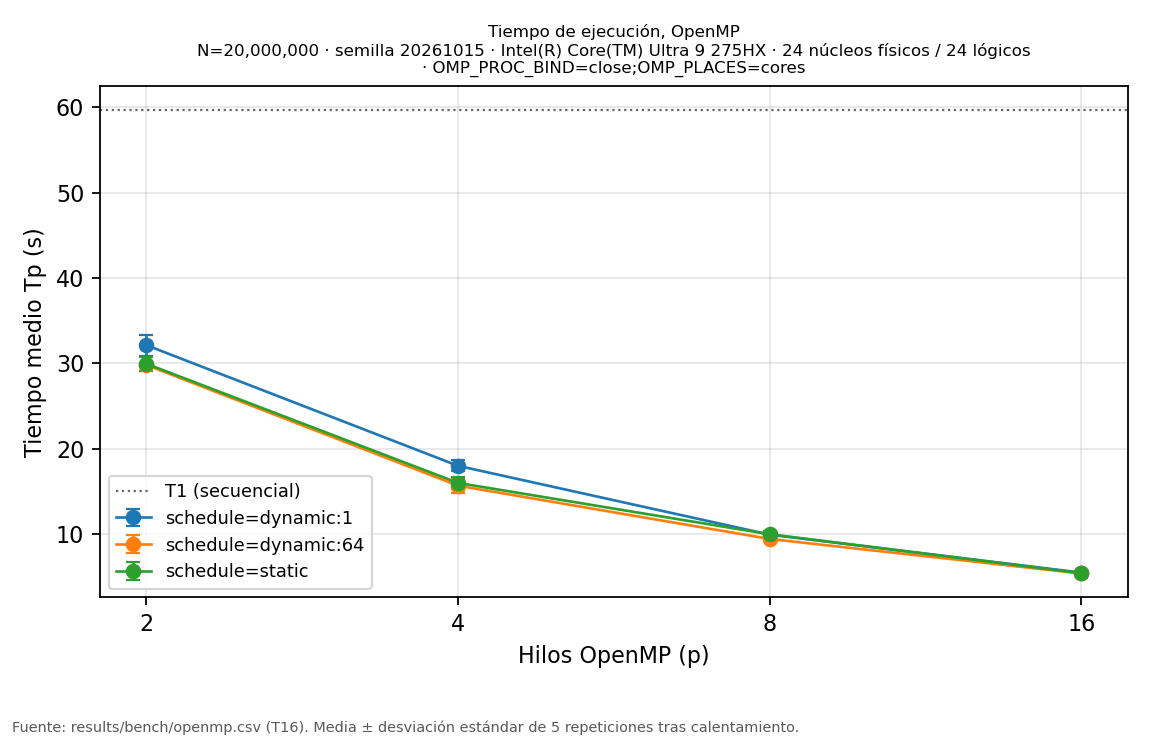
\includegraphics[width=\columnwidth]{openmp_tiempo.png}
\caption{Tiempo de pared OpenMP frente al número de hilos, con la referencia $T_1$; barras de error de una desviación estándar.}
\label{fig:openmp-tiempo}
\end{figure}

\begin{figure}[!t]
\centering
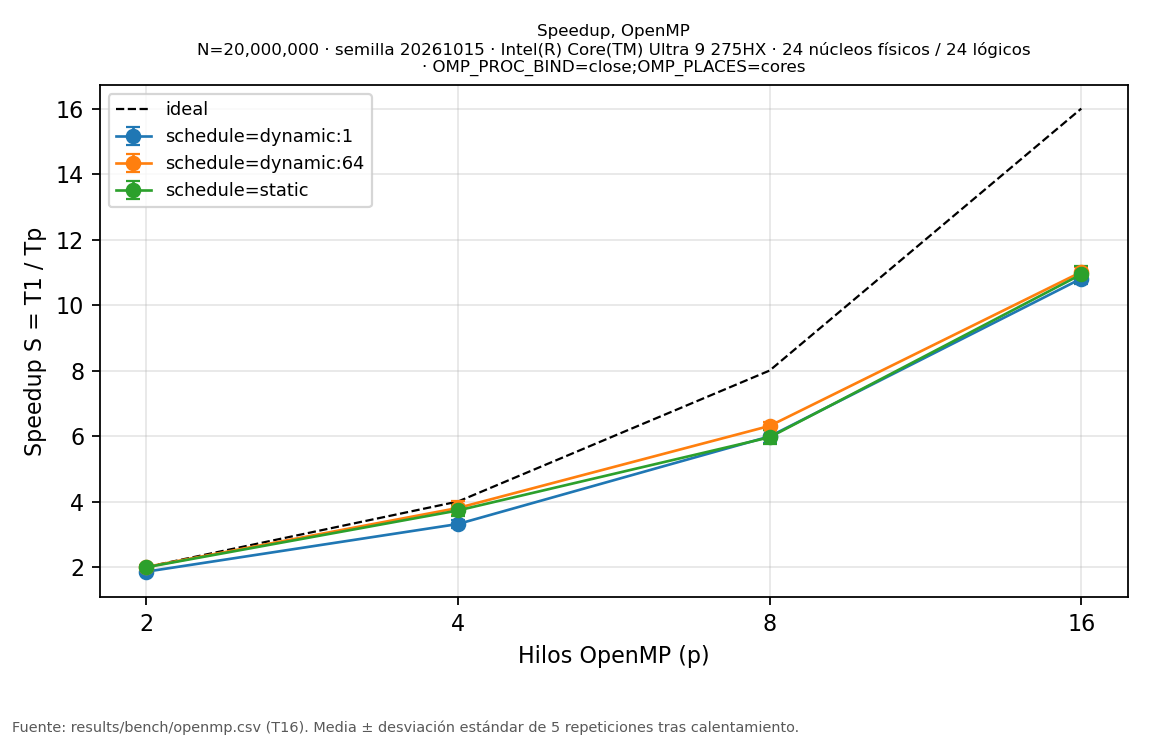
\includegraphics[width=\columnwidth]{openmp_speedup.png}
\caption{Speedup OpenMP por \emph{schedule}, con la recta ideal $S_p = p$.}
\label{fig:openmp-speedup}
\end{figure}

\begin{figure}[!t]
\centering
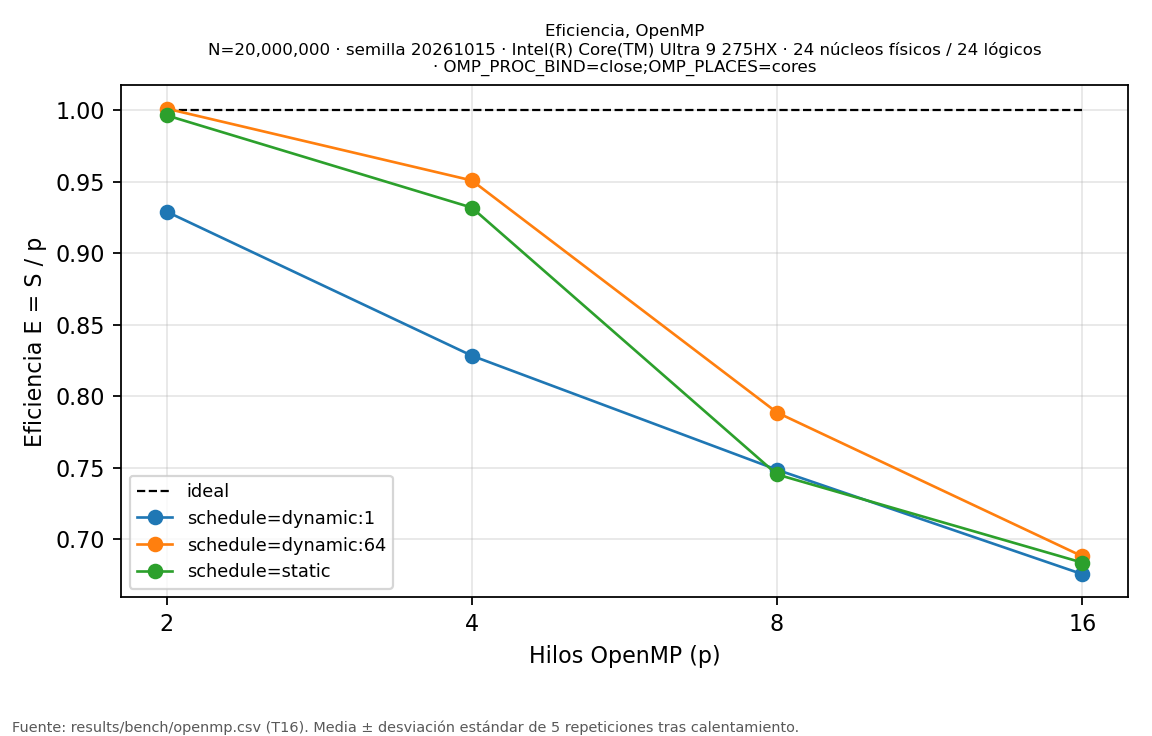
\includegraphics[width=\columnwidth]{openmp_eficiencia.png}
\caption{Eficiencia OpenMP por \emph{schedule}, con la referencia ideal $E_p = 1$.}
\label{fig:openmp-eficiencia}
\end{figure}

Con 2 y 4 hilos el speedup es casi lineal con \codigo{static} y \codigo{dynamic:64} ($E_p \ge 0{,}93$). Con 16 hilos los tres \emph{schedules} convergen a un speedup de 10,8--11,0 y una eficiencia de 0,68--0,69; el mejor punto es \codigo{dynamic:64}, con $S_{16} = 11{,}01$ y un throughput de \num{3.69e6} escenarios por segundo.

\codigo{dynamic:1} es el más lento con pocos hilos ($S_2 = 1{,}86$, $e_2 = 0{,}076$). Cada iteración dura unos \qty{3}{\micro\second}, por lo que repartir una iteración por solicitud hace que el costo de planificación de OpenMP sea apreciable; con bloques de 64 iteraciones ese costo se amortiza y el desequilibrio residual es despreciable, porque todas las temporadas tienen el mismo número de días. Con 8 hilos \codigo{dynamic:64} sigue siendo cerca de un 5\,\% más rápido que los otros dos; con 16 la diferencia entre \emph{schedules} baja a menos de un 2\,\%.

La fracción serial de Karp--Flatt no es monótona: crece hasta 8 hilos ($e_8 \approx 0{,}04$--$0{,}05$) y \emph{disminuye} con 16 ($e_{16} \approx 0{,}03$). Una fracción serial fija o una sobrecarga creciente de OpenMP harían que $e_p$ fuese constante o creciente. La explicación más consistente con el hardware es la heterogeneidad de núcleos: el equipo tiene 8 núcleos P, y a partir de 8 hilos parte del trabajo puede caer en núcleos E más lentos, de modo que $p$ hilos no equivalen a $p$ núcleos de igual capacidad. Por eso la pérdida de eficiencia entre 4 y 16 hilos no debe atribuirse solo a OpenMP. El bucle no comparte memoria ni sincroniza hilos dentro de la región, lo que es coherente con que el costo de la reducción final (un histograma de \qty{4}{\kilo\byte} por hilo) sea pequeño frente a segundos de cómputo.
% TODO-T33: confirmar la hipótesis P/E con una corrida de 8 hilos fijados a núcleos P (o con la medida por núcleo) antes de afirmarla en las conclusiones.

\subsection{OpenMP en el equipo 2}

Como contraste, el equipo~2 (6 núcleos físicos, 12 lógicos) midió $T_1 = \qty{71.01}{\second}$ (desviación \qty{0.57}{\second}) con la misma carga y obtuvo el mismo $k$. Con \codigo{static} logró speedups de 1,87, 3,39, 5,68 y 6,67 para 2, 4, 8 y 16 hilos, y con \codigo{dynamic:64}, de 1,89, 3,44, 5,96 y 7,32. Los puntos de 8 y 16 hilos están sobresuscritos ---16 hilos superan incluso los 12 lógicos---, por lo que la ganancia por encima de 6 hilos proviene de la ejecución simultánea en núcleos lógicos y no de núcleos adicionales; esos puntos no se usan para calcular eficiencia.

\subsection{MPI, híbrido y experimentos X1--X3}

% TODO-T33: insertar aquí, desde results/bench/mpi.csv, results/bench/hibrido.csv y los CSV de X1--X3:
%   (a) Tabla MPI E1 y E2 con 2/4/8/16 procesos: T_p ± desv., S_p, E_p, e_p, nodos y distribución por nodo.
%   (b) Tabla híbrido 2/4/8/16 núcleos totales con al menos dos factorizaciones P×T por presupuesto.
%   (c) X1 escalabilidad fuerte (N = 2×10^8) OpenMP vs. MPI vs. híbrido en el Swarm de tres equipos; figura de speedup y de Karp–Flatt.
%   (d) X2 escalabilidad débil (carga proporcional a p) con eficiencia de Gustafson.
%   (e) X3 barrido N = 10^6…10^9: tiempo y throughput frente a N; peso del costo fijo.
%   (f) X4 / T32: E1 frente a E2 con los mismos procesos en nodos heterogéneos (hipótesis H2).
%   Figuras esperadas: results/figures/mpi_*.png, hibrido_*.png, x1_*.png, x2_*.png, x3_*.png.
\textit{[Pendiente: resultados de MPI E1/E2, híbrido y experimentos X1--X4 en el clúster de tres equipos.]}

\section{Resultados científicos}
\label{sec:resultados}

Esta sección presenta los productos de la campaña oficial X6 sobre las 5 estaciones de trabajo, los 2 regímenes, las 13 capacidades de drenaje y los $K = 100$ conjuntos bootstrap.

\textbf{Advertencia sobre la validez del generador.} La validación V6 frente a las series observadas no se cumple en los estadísticos de cola (Sección~\ref{sec:metodologia}): el generador reproduce la frecuencia de días lluviosos, la media de los montos y la longitud de las rachas, pero subestima la desviación y los percentiles altos de la lluvia diaria. Mientras no se resuelva, las probabilidades de esta sección deben leerse como cotas inferiores del riesgo, sobre todo en las capacidades de drenaje altas, donde la inundación depende de eventos extremos.
% TODO-V6: actualizar esta advertencia con el resultado final de la Ola D (docs/validacion-v6.md).

\subsection{Probabilidad de inundación por zona, capacidad y régimen}

% TODO-T35: tabla desde el CSV de X6 (scripts/run/analizar-riesgo.py): por estación × régimen × C,
%   p_hat, intervalo de Wilson al 95 % y banda epistémica P5–P95 entre los 100 conjuntos bootstrap.
%   Si la tabla completa no cabe, mostrar C = 5, 15, 25, 35 y 65 mm/día y llevar el resto a un anexo.
\textit{[Pendiente: tabla de $\phat$ con IC de Wilson y banda epistémica, T35.]}

\subsection{Curva riesgo--capacidad}

% TODO-T35: figura results/figures/riesgo_capacidad_*.png (una curva por estación, paneles normal / El Niño,
%   banda epistémica sombreada) y tabla de la capacidad mínima C* que cumple p_hat <= 10 %, interpolada.
\textit{[Pendiente: curvas riesgo--capacidad y capacidad mínima $C^{*}$ para $\phat \le 10$\,\%, T35.]}

\subsection{Curva de excedencia del máximo acumulado}

% TODO-T35: curva P(A_max > a) a partir del histograma de 512 clases, por estación y régimen, en escala log.
\textit{[Pendiente: curvas de excedencia de $\Amax$, T35.]}

\subsection{Año normal frente a año El Niño}

% TODO-T35: cociente p_hat(El Niño) / p_hat(normal) por estación y capacidad, con su incertidumbre;
%   contrastar el mecanismo de cantidad de lluvia (costa norte) con el de capacidad de drenaje (Chosica).
\textit{[Pendiente: comparación entre regímenes, T35.]}

\section{Análisis de sensibilidad}
\label{sec:sensibilidad}

El experimento X7 evalúa cuánto dependen las conclusiones de los supuestos de diseño que no provienen de mediciones de campo: el umbral crítico $U$ y el régimen climático. Se repite la estimación de la Sección~\ref{sec:resultados} con $U = 30$, 50 y \qty{80}{\milli\metre}, manteniendo la semilla y los conjuntos bootstrap, de modo que las diferencias entre umbrales no se confunden con ruido de muestreo.

% TODO-T42: desde los CSV de scripts/run/sensibilidad.py:
%   (a) figura de p_hat frente a C para U = 30 / 50 / 80 mm, por estación y régimen;
%   (b) tabla del desplazamiento de la capacidad mínima C* al cambiar U;
%   (c) efecto del régimen (normal / El Niño) para cada U.
\textit{[Pendiente: sensibilidad al umbral $U$ y al régimen, T42.]}

La sensibilidad se interpreta con la misma salvedad de V6 que la Sección~\ref{sec:resultados}: un generador que subestima la cola tiende a subestimar el riesgo, y el sesgo crece con $U$, porque un umbral mayor solo se supera con eventos más extremos.
% TODO-V6: revisar este párrafo cuando la Ola D cierre el diagnóstico de V6.

\section{Conclusiones}
\label{sec:conclusiones}

% TODO-T46: redactar cuando estén T33, T35, T42 y V6. Una conclusión por pregunta y por criterio, cada una con su evidencia:
%   (1) correctitud: V1/V3/V4/V5 aprobadas; equivalencia bit a bit en todos los backends gracias a Philox;
%   (2) rendimiento OpenMP, MPI E1/E2 e híbrido (speedup, eficiencia, Karp–Flatt) y límites del hardware P/E;
%   (3) E1 frente a E2 en nodos heterogéneos (H2);
%   (4) riesgo por zona y régimen, capacidad mínima C* y efecto de El Niño;
%   (5) limitaciones: V6 en la cola, modelo no hidráulico, CUDA en desarrollo (EXT1/EXT2); trabajo futuro (variante scan de Lindley).
\textit{[Pendiente: conclusiones, T46.]}


\bibliographystyle{IEEEtran}
\bibliography{referencias}

\end{document}
